\documentclass{article}

\usepackage{times}
\usepackage[top=1in, bottom=1in, left=1in, right=1in]{geometry}
\usepackage{graphicx}
\usepackage{listings}
\lstset{language=C}
\lstset{numbers=left, numberstyle=\small, stepnumber=1, numbersep=5pt, breaklines=true}
\usepackage{upquote}
\usepackage{color}
\usepackage{xcolor}
\usepackage{caption}
\usepackage{fixltx2e}

\DeclareCaptionFont{white}{\color{white}}
\DeclareCaptionFormat{listing}{\colorbox{gray}{\parbox{\textwidth}{#1#2#3}}}
\captionsetup[lstlisting]{format=listing,labelfont=white,textfont=white}

\DeclareCaptionFormat{figure}{\colorbox{gray}{\parbox{\textwidth}{#1#2#3}}}
\captionsetup[figure]{format=listing,labelfont=white,textfont=white}

\begin{document}

\author{Joshua Ashby\\
        Maurice Ashby\\
        Linux And Sci\\
        \texttt{http://joshashby.com}\\
	\texttt{joshuaashby@joshashby.com}
}
\title{Project: Bouncing Off Bumpers}

  \begin{center}
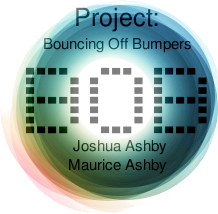
\includegraphics{boblogo}\\
\texttt{http://bob.joshashby.com}\\

In Conjunction with:\\

\includegraphics{logo-med}\\
\texttt{http://joshashby.com}\\
  \end{center}

\maketitle
\abstract{Bouncing off Bumpers, or BOB is a competition robot built by Joshua Ashby and his grandfather Maurice Ashby for the April 15th, 2009 Sparkfun Autonomous Vehicle Competition. It measures approximately 3 feet long by 2 feet wide by 2 feet tall; it weights approximately 50 pounds without the battery and electronics.
This paper will go into detail about the many systems involved in the build process of BOB, and provide insight into how many of these systems were designed, and the logic behind them (Please note that this paper is always going to be changing, and the data could easily change the day after the latest pubilishing).\\
As of April 17th 2010, BOB has also competed in the 2010 Sparkfun AVC and won the Kill Switch award, however due to both a programming bug and hardware issue, he would not turn left and as a result was not able to get around the building, only 10\%.}\\

\newpage
\tableofcontents
\listoffigures
\renewcommand{\lstlistlistingname}{List of Files \& Examples}
\lstlistoflistings

\newpage

\section{Revisions}\\
March 10th/11th/12th, 2010 - Joshua Ashby\\
Added more to the electronics, Motor controller node part to include the new Quad Low-side V1.5.1 through Revision 3 boards.\\
April 19th, 2010 - Joshua Ashby\\
Added even more to the new sections, cleaning it up, and overall re-writing some parts for better understanding. Rewrote software section also.\\
April 20th, 2010 - Joshua Ashby\\
Finished the software section and got the appendix of code cleaned up. also changed the program boxes from floats to listings. Still need to fix the steering descriptor section (marked with TODO).\\
November 11th, 2010 - Joshua Ashby\\
Started work on updating the various sections and the hardware section for the new boards and matching code. Updated Linux And Sci logo.\\
November 12-13th, 2010 - Joshua Ashby\\
Added the Current Generation section, and a more in depth discussion of the electronic. Also went through and did some clean up, still a lot to do. Moved abstract to the title page.\\

\newpage

\section{Introduction and Background}
The electronics were designed by me (Joshua Ashby), and built by me along with the aid of my grandfather Maurice Ashby. As of March 10th, 2010 BOB is running on the newly designed and completed Generation 3 electronics. These electronics include the "Taco" Quad-Motor Motor controller board with a few minor additions to the board, along with several other minor boards. Over all the design process for the electronics have taken the longest as the motor controllers must be able to meet the demand of 10A per motor, as a result several generation of electronics have gone out the window.\\
As of November 11th 2010, design on the Generation 4 electronics has been started. These boards are regressing to the multiple "Nodes" consisting of the main brain node, or Master Node, two "dead\footnote{Dead in this sense means these nodes do not have any programmable intellegence on them. They are useless without the Master Node.}" motor controller nodes.\\
The mechanics of the robot, which refers to the frame and body, the steering and related mechanisms, and the propulsion system were designed and built by us over a course of approximately 5 weeks, and has not had any major problems besides the replacement of the front motor.\\
\section{Platform\footnote{Please note, the frame was made to be cheap, and need little maintanince}%
}
\subsection{Shape, Design and Material}
In order to build the frame in both a time and cost effective way, we choose to reuse some old square steel tubing that measures  and has a wall thickness of. My grandfather had just enough laying around his shop to build a frame with. By using steel square tubing, and welding the joints, we were able to build a sturdy frame capable of carrying well over 100LBS over rough terrain.\\
The design of a three wheeled robot came after evaluating the cost of the wheels that would be used; to keep the cost down, only three wheels would be used. Because only three wheels would be used, the frame would have to be built in a fashion that did not promote tilting when the robot turns but still allow a large amount of room to build on top of. To accomplish this, an elongated pentagon design was created. The main drive wheel would be placed at the back of the robot in a triangle shaped portion of the frame, while the middle and front of the body would be a square shape, with two wheels in the front to steer with.\\
\subsection{Steering}
The steering for BOB was modeled after a car style steering system, where two wheels are connected via a rod which is in turn moved left or right to turn the wheels (Figure \ref{steering}).
\begin{figure}[htp]
  \begin{center}
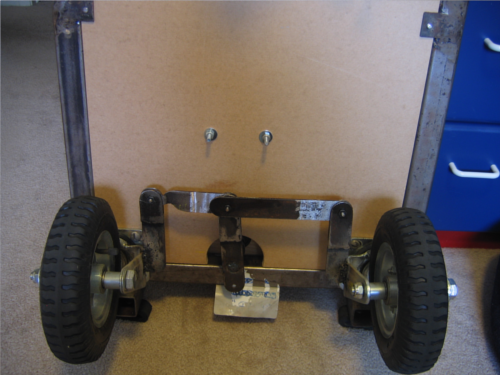
\includegraphics[scale=0.5]{steering}
  \end{center}
  \caption{Example of the steering build used}
\label{steering}
\end{figure}\\
TODO: Fix this description\\
The build of this was accomplished by using two pre-built wheel casters, and welding on strips of quarter inch thick steel. These strips are approximately 6 inches long, and at the end that is not welded to the caster wheels, there is a hole drilled. Then connecting the two wheels via these strips, is a second pair of steel strips that are hooked up to the steering motor.\\
The steering motor is a 9.6V 10A drill motor that has been mounted with a right angle drive. This allows the motor to lay flat with the robot frame and still be able to turn the steering rod (Figure \ref{steeringmotor}).
\begin{figure}[htp]
  \begin{center}
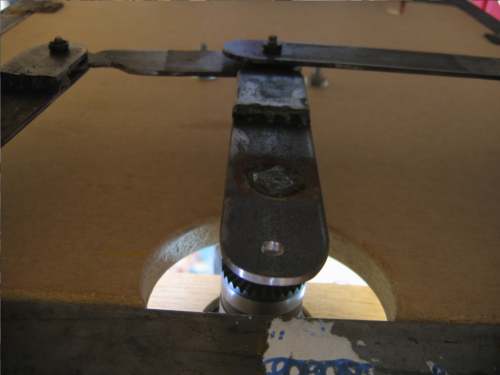
\includegraphics[scale=0.5]{steeringmotor}
  \end{center}
  \caption{Example of the steering motor}
\label{steeringmotor}
\end{figure}\\
One problem that we did not foresee while building the steering, is the ability to drive straight. Because the steering mechanism does not have a method of straighting its self out quickly and effectivly, a new task is introduced to the electronics and programming until further improvments to the steering can be made. This may be accomplished by turning the front motor into an mechanism much like a servo through the use of programming and the ability of the motor controllers, however as of right now, thing has been done to take care of this problem.\\
\subsection{Propulsion}
Transferring power from the drill motor to the back drive wheel was one of the greatest technical difficulties we encountered. We started off by testing the idea of a friction drive. This style of drive has the motor running parallel to the wheel, and the output shaft using friction to turn the wheel. This worked great going downhill, but as soon as the drive had a load to pull, such as on flat ground, or uphill, the drive would start to slip.\\
Our second attempt was based off of a bike, just instead of a chain drive, we decided to do a belt drive as my grandfather had many of the needed parts. The motor was mounted perpendicular to the rotating axis of the wheel, and had a small 1.25 inch radius belt pulley on it. The wheel then had a larger, 2 inch radius, belt pulley on it. The two pulleys were connected via 8 inch diameter cogged belt. The axle for the motor is a milled axle that is supported by a bearing block at one end. The other end is tapered down to allow it to fit in the motor chuck. This also allows the motor to be disconnected from the axle, allowing the robot to be moved around with out power to the motor. (Figure \ref{reardrive}).
\begin{figure}[htp]
  \begin{center}
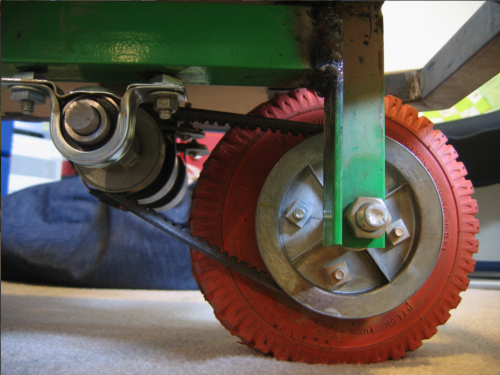
\includegraphics[scale=0.5]{reardrive}
  \end{center}
  \caption{Example of the drive system used}
\label{reardrive}
\end{figure}\\
This drive system worked perfectly both downhill and uphill, and as a result it is the drive system currently used. The motor is the same as the steering motor, a recycled drill motor that is rated at 9.6V and 10A.\\
\section{Electronics - Introduction \& History}
\subsection{Introduction}
The electronics have always been a troublesome matter for this project and as this is being typed, the electronics still are providing issues, even with new designs.\\
The motors, which each draw ~10A, must have easy to use, and cheap to build motor controllers, along with the ability to easily replace major parts while the robot is not in the Lab or near a soldering iron. This means the motor controllers can not be store bought, as all of the quality controllers that we can find are not only expensive, but also do not have common, easy to find parts. Instead to replace a part, the whole controller must be replaced most the time\footnote{Plus it's funner to build your own controllers}.\\
Generation 1 electronics consisted of one micro-controller, and one and a half motor controllers. These electronics shorted out at the 2009 Sparkfun AVC competition, and as a result will only be used as both a comparison, and as a resource for what not to do on future generations.\\
Please note that voltages will always be expressed like so: V\textsubscript{5} or V\textsubscript{12} Due to the mixed voltages that exsist on BOB.
\subsection{Motor controller - History}
As stated above, the use of store bought motor controllers is out of the question for use on BOB. They tend to be expensive, and typically must have the whole unit replaced if something burns out. Because of this, the motor controllers have been hand designed by us.\\
\subsubsection{Generation 1}
The first version, which is the version that was used during the 2009 Sparkfun AVC competition, was designed to be very simple, and yet still provide the power that was needed for the motors. It consisted of a TIP125 PNP transistor driving a pair of paralleled IRF540N n-channel MOSFETs. At the time of their designing and building, we both were very new to MOSFETs and as a result the knowledge of how to hook the MOSFETs up, and the voltage required to drive them was unknown. This caused many problems, such as the MOSFETs not having enough voltage and amperes for them to fully close. This caused them to over heat, and also caused a massive power spike somewhere along the lines that burnt out the MOSFETs and transistor.\\
\subsubsection{Generation 2}
The new generation 2 motor controllers were designed to avoid these problems, along with begin to merge into a modular system. These new motor controllers were called the Motor Nodes, and included two motor controllers, and a micro-controller that talked to the controllers. The micro-controller for generation 2 electronics was an Atmega328p which took care of both the sensors and the motor controllers. The basic design of using the transistors to switch the logic level were used, but with a few improvments such as temperature shut off for the MOSFETs, however it was discovered in late December 2009 that this method of driving the MOSFETs was not atiquate enough, and as a result this method is no longer used. For this reason the Generation 2 electronics have been ditched and new Generation 3 electronics designed and put in place.\\
\subsubsection{Generation 3}
The Generation 3 board consists of the main ATmega328P running at 5V with a 16MHz crystal. The I2C headers are broken out\footnote{Which also provide two analog pins for the ultrasounds on BOB}, and the ATmega has 2 LEDs connected to PortD pins 3 and 5, also known as OC2B and OC0B. This allows for PWM debugging of any functions. Next the Atmega is connected to two TC4424CPA chips, one of these chips being on PD1 and PD2, OR1A, OR1B for PWM speed control, and the other chip being on pins PD2, PD4 for simple digital triggering of relays.\\
This board, which is named Taco is infact a general purpose MOSFET board, but has been desinged in conjunction with BOB for use on him, however the only problem so far has been the traces not being big enough to carry the 10A and 20A from the motors. As a result the board also has several high amperage wires for the MOSFETs and motor outputs.\\
The I2C header is broken out which I2C on the Atmega328p is the analog pins 4 and 5, which means that the board can also be used for analog inputs, such as was used for the ultrasounds on BOB.\\
Each motor controller board is the same design since they both serve similar motors. As a result they have the MOSFETs for the motor and it's corisponding dirrection relay. Future versions may bring in the temperature shut off for the MOSFETs however this feature is currently not going to be on the Generation 4 boards for technical reasons.\\
Along with the new MOSFET drivers that were introduced in Generation 3 electronics, the MOSFET gates have current limiting resistors, and 12V zener diodes to prevent power spikes. The boards also have a 10uF and 1000uF capacitor to help smooth out power drops from the motors.\\
\subsection{Power Node}
The Power Node, as of Generation 2 electronics is simply a “dead” Node as one might call it. It has no intelligence, instead it's only function for generation 2 is to regulate and distribute 5V to all the boards. It does this via Molex connectors off of old ATX power supplies from computers. This same board design was used in the Generation 3 electronics also.\\
\section{Current Generation - Generation 4}
Generation 4 electronics are in some ways a stepping stone. They place the electronics into an area where they may be broken up into intelligent Nodes, while at the same time, keeping the same principle of operation the same and being based off the same electronics as Generation 3.\\
\subsection{Master Node}
As stated above, there are three nodes that will end up on BOB once Generation 4 electronics are completed. Of these three nodes, the Master Node is the only node which is capable of operation on it's own. This means that it has the microcontroller on board, while the other two nodes are simply additional boards which allow the Master Node to interact with the motors.\\
The controller of choice for the Master Node is still the Atmega328p for the time being. This is because not only are all of my libraries and code already written and specialized for the AtmegaXX8 family, but I also currently have the most experience in working with these chips. The Atmega328p gives 32K of flash memory to work with, so my larger and inefficient libraries are okay, seeing as they currently come out to be aproximentally 13K with little optimization. The chips also provide 6 PWM\footnote{PWM- Pulse Width Modification - fancy use of really fast digital signals to, in the case of it's use on BOB, emulate an analog signal} outputs, and plenty of digital inputs and outputs, along with 6 analog inputs, 2 of which, however, are used for I2C communication. Through the plethora of inputs and outputs and memory which the Atmega328p provides me with, I can easily run all of BOB off of one chip.\\
The Atmega328p has all it's pins broken out into .01 inch spaced headers, for easy access during development and debuging. It also has an Atmel 6 pin ISP header broken out, and a 4 pin I2C header broken out. The I2C header pins are arranged in the following confiuguration:\\
\\
\begin{tabular}{ l | l | l | l }
V\textsubscript{5} & SDA & SCL & Gnd \\
\end{tabular}\\
\\
The Atmega also has 4 of it's pins broken out into a 2 by 5 pin header that is used for communication to the Motor Nodes. There is a ribbon cable that then connects the Master Node to both Motor Nodes via this 2x5 header. The pin out is as followed:\\
\\
\begin{tabular}{ l | l | l | l | l }
V\textsubscript{12} & V\textsubscript{5} & Pwm-Back & Digital-Back & Gnd \\
V\textsubscript{12} & V\textsubscript{5} & Pwm-Front & Digital-Front & Gnd \\
\end{tabular}\\
\\
In addition to the Atmega, the Maste Node is also the power distribution node. It has the on board 5V regulator and filters which is then distributed to the other nodes where needed.\\
\subsection{Motor Nodes}
The Motor Nodes are simply all the electronics which directly deal with interacting with the motors. They contain the IRF540N N-channel MOSFETs which handle the voltage and amperage of the motors, and the switching MOSFETS, also IRF540N's which handle the switching of the heavy duty relays which take the place of an H-Bridge.\\
The motor MOSFETs are driven by the TCP4424 N-channel 3A dual MOSFET driver chip, which takes the 5V PWM logic of the Atmega and converts it to the 12V logic of the MOSFETS, and also takes care of charging and driving the MOSFETs gates. This chip has been in use since Generation 3 electronics, and has proven to be indispensable to the operation of BOB. These chips also handle the PWM signal very well, and allow for effective speed control of BOB through the use of PWM. Also, above the MOSFETs is a small fan which takes care of heat problems that occur at slower speeds where the MOSFET's are burning off restricted amps that are being pulled through it, as heat.\\
To manage switching the dirrection of the motors, in Generation 1 a mechanical solution was devised, a Double Pull, Double Throw "Ice cube\footnote{They are called Ice Cube relays because of the large box shape and clear plastic which surrounds the relay itself.}" relay would be used, wired in an alternating pattern so that when the relay was activated, the pins of the motor are effectivly switched, changing the dirrection of the motor. Since the relay's coil pulls more current than the Atmega can safely source, a MOSFET is used to take care of the switching process. Since this MOSFET is not handling large amounts of current, or being used all the time, it does not need a heat sink or to be dirrectly under the fan, however the design of the Nodes has the MOSFET next to the motor MOSFET in any case.\\
\section{Software}
\subsection{Libraries - Introduction}
As of January 2010, BOB runs a custom writen library set that takes care of everything from PWM and digital function to analog, ultrasounds, and calibration. Newer additions to this library include (or will soon include) I2C functionality.\footnote{Please note that memory was not an issue during the time of the writing of these libraries there for they have many places that memory types can be changed to improve file size.}\\
\subsection{Digital Functions}
First up is the digital function library (Page: \pageref{digital}). The digital function library takes care of turning a pin on or off, which seems simple enough. While this task is quite trivial in code, those few extra lines tend to make the code look messy, which I don't like as much.\\
\begin{verbatim}void portB_out(int pin, int value)\end{verbatim}
Simply send the pin number (0 through 7), and the value (1 or 0) and the corrisponding pin on PORTB will be set to that value.\\
\begin{verbatim}void portD_out(int pin, int value)\end{verbatim}
Simply send the pin number (0 through 7), and the value (1 or 0) and the corrisponding pin on PORTD will be set to that value.\\
\begin{verbatim}void out(char port, int pin, int value)\end{verbatim}
Send the port letter, the pin number, and the value (0 or 1) and the corrisponding pin on that port will be set to that value.\\
\subsubsection{Example}
\begin{lstlisting}[caption={Digital examples},label=digitalex,frame=bl]
portB_out(3,1); //will turn on (close) PORTB pin 3
portD_out(0,0); //will turn off (open) PORTD pin 0
out('D',5,1); //will turn on (close) PORTD pin 5
\end{lstlisting}

\subsection{Analog Functions}
Unlike the digital code, reading from an analog pin takes some work. First you have to setup the registers, which in my case get me going at a prescaler of 128, interupt driven, and left alinged bits. The left aligned results mean that I don't have to do fancy code and get 10bit results, which I don't need. instead I can simply read the ADCH register and get an 8 bit result. The next step is to read the results, or change the pin that I am reading from, both which take more code. As a result of all this, placing the analog functions inside of a nice, clean library makes sense (Page: \pageref{analog}).\\
\begin{verbatim}void adc_start(void)\end{verbatim}
Calling this will simply setup the correct registers, and start an interupt driven ADC comversion. After this is called the value of the ADC can be found in the ADCH register.
\begin{verbatim}void adc_stop()\end{verbatim}
Simply stops the ADC conversions.
\begin{verbatim}void adc_change(int chan)\end{verbatim}
Calling this with pins numbers 0-8 will cause the ADC to be stoped, the pin changed, and the ADC started again.
\subsubsection{Example}
\begin{lstlisting}[caption={Analog examples},label=analogex,frame=bl]
adc_start();
adc_stop();
adc_change(3);
\end{lstlisting}

\subsection{PWM Functions}
Like the analog functions, the PWM functions that I needed were large, and very messy pieces of code. They consisted of several functions that setup the registers for the three PWM timers, and then several more to add in functions like ramp up and down functionability. (Page: \pageref{pwm}).
\begin{verbatim}(#L)\end{verbatim} stands for number and letter respectivly, when used likst this it means too replace \begin{verbatim}(#L)\end{verbatim} with something such as 0A or 2B.
\begin{verbatim}void pwm_setup_all(void)\end{verbatim}
sets up the registers for all the PWM timers in phase correct not prescaled PWM mode.
\begin{verbatim}void pwm_setup(#)(void)\end{verbatim}
Sets up the given PWM channel timer with the corrent register settings.
\begin{verbatim}void pwm(#L)(unsigned int value)\end{verbatim}Tests the turning motor and functions, simply goes through and cycles which direction every time.
Sets the PWM duty cycle of the given channel.
\begin{verbatim}void pwm_ramp(#L)(unsigned int value, unsigned int speed)\end{verbatim}
Ramps the given PWM channel at the given speed to the given duty cycle.
\begin{verbatim}void pwm_rampUp(#L)(unsigned int value, unsigned int speed)\end{verbatim}
Ramps up the given PWM channel at the given speed to the given duty cycle.
\begin{verbatim}void pwm_rampDown(#L)(unsigned int value, unsigned int speed)\end{verbatim}
Ramps down the given PWM channel at the given speed to the given duty cycle.
\subsubsection{Example}
\begin{lstlisting}[caption={PWM examples},label=pwmex,frame=bl]
pwm_setup_all(); //setup all the PWM timers
pwm2A(50); //sets OCR2A to 50
pwm_ramp1A(255, 10); //will ramp OCR1A to 255 with a delay of 10ms between each step

\end{lstlisting}

\subsection{Robotics Functions}
The robotics library takes care of most of the things that BOB needs to run. It houses the turn functions, and the filter that takes care of the  ultrasound data. This filter is a custom rolling average with a few additions which smooth the data points out really well as the analog outputs on the ultrasounds are a little jumpy (Page: \pageref{robot}).\\
\begin{verbatim}void turn_left(void)\end{verbatim}
Does exactly what it says, simply takes care of the timing and everything for turning.
\begin{verbatim}void turn_right(void)\end{verbatim}
Same as turn left.
\begin{verbatim}void stop(void)\end{verbatim}
Stops everything and displays the error 1.
\begin{verbatim}void calibrate(void)\end{verbatim}
Calling this starts the ADC, then fills the rolling average, setting the base length to the first set of data from when the bots not moving, very useful and when used with the filter makes nice data for BOB.
\begin{verbatim}void ultrasound_test(void)\end{verbatim}
Tests the ultrasounds and displays the results with the on board LEDs
\begin{verbatim}int ultrasound_filter(int pin)\end{verbatim}
Starts a rolling average with a few additions to smooth out data points, returns the current average.
\begin{verbatim}void test_turn(void)\end{verbatim}
Tests the turning motor and functions, simply goes through and cycles which direction every time.
\begin{verbatim}void test_motor(void)\end{verbatim}
Tests the main propulsion motor and functions, simply goes through and cycles which direction every time.
\subsubsection{Example}
\begin{lstlisting}[caption={Robot examples},label=robotex,frame=bl]
turn_left();
turn_right();
pwm2B(ultrasoundfilter(4)); //will cause the PWM 2B channel to be set to
//whatever the returned value of ultrasoundfilter is
\end{lstlisting}

\subsection{Boot Functions}
Finally the boot library takes care of setting everything up as the robot first starts, basically it's an implementation of a low level bios for BOB (Page: \pageref{boot}).\\
\begin{verbatim}void bios(void)\end{verbatim}
Calling this will setup everything that BOB needs to run, calibrates the sensors and in general gets everything ready.
\begin{verbatim}void all_good(void)\end{verbatim}
Status LED on.
\begin{verbatim}void oh_crap(void)\end{verbatim}
Status LED off.
\begin{verbatim}void error(int type)\end{verbatim}
gives a few different types of errors that can be given through the LEDs, not really used all the much yet.
\subsubsection{Example}
\begin{lstlisting}[caption={Boot examples},label=bootex,frame=bl]
bios(); //sets up everything needed for BOB to run
error(1); //will display the error 1
\end{lstlisting}

\newpage
\section{About the builders}
\subsection{Joshua Ashby}
\begin{figure}[htp]
  \begin{center}

\includegraphics[scale=0.05]{josh}
  \end{center}
  \caption{Author and co-builder Josh Ashby}
\label{josh}
\end{figure}\\
\subsection{Maurice Ashby}
\begin{figure}[htp]
  \begin{center}
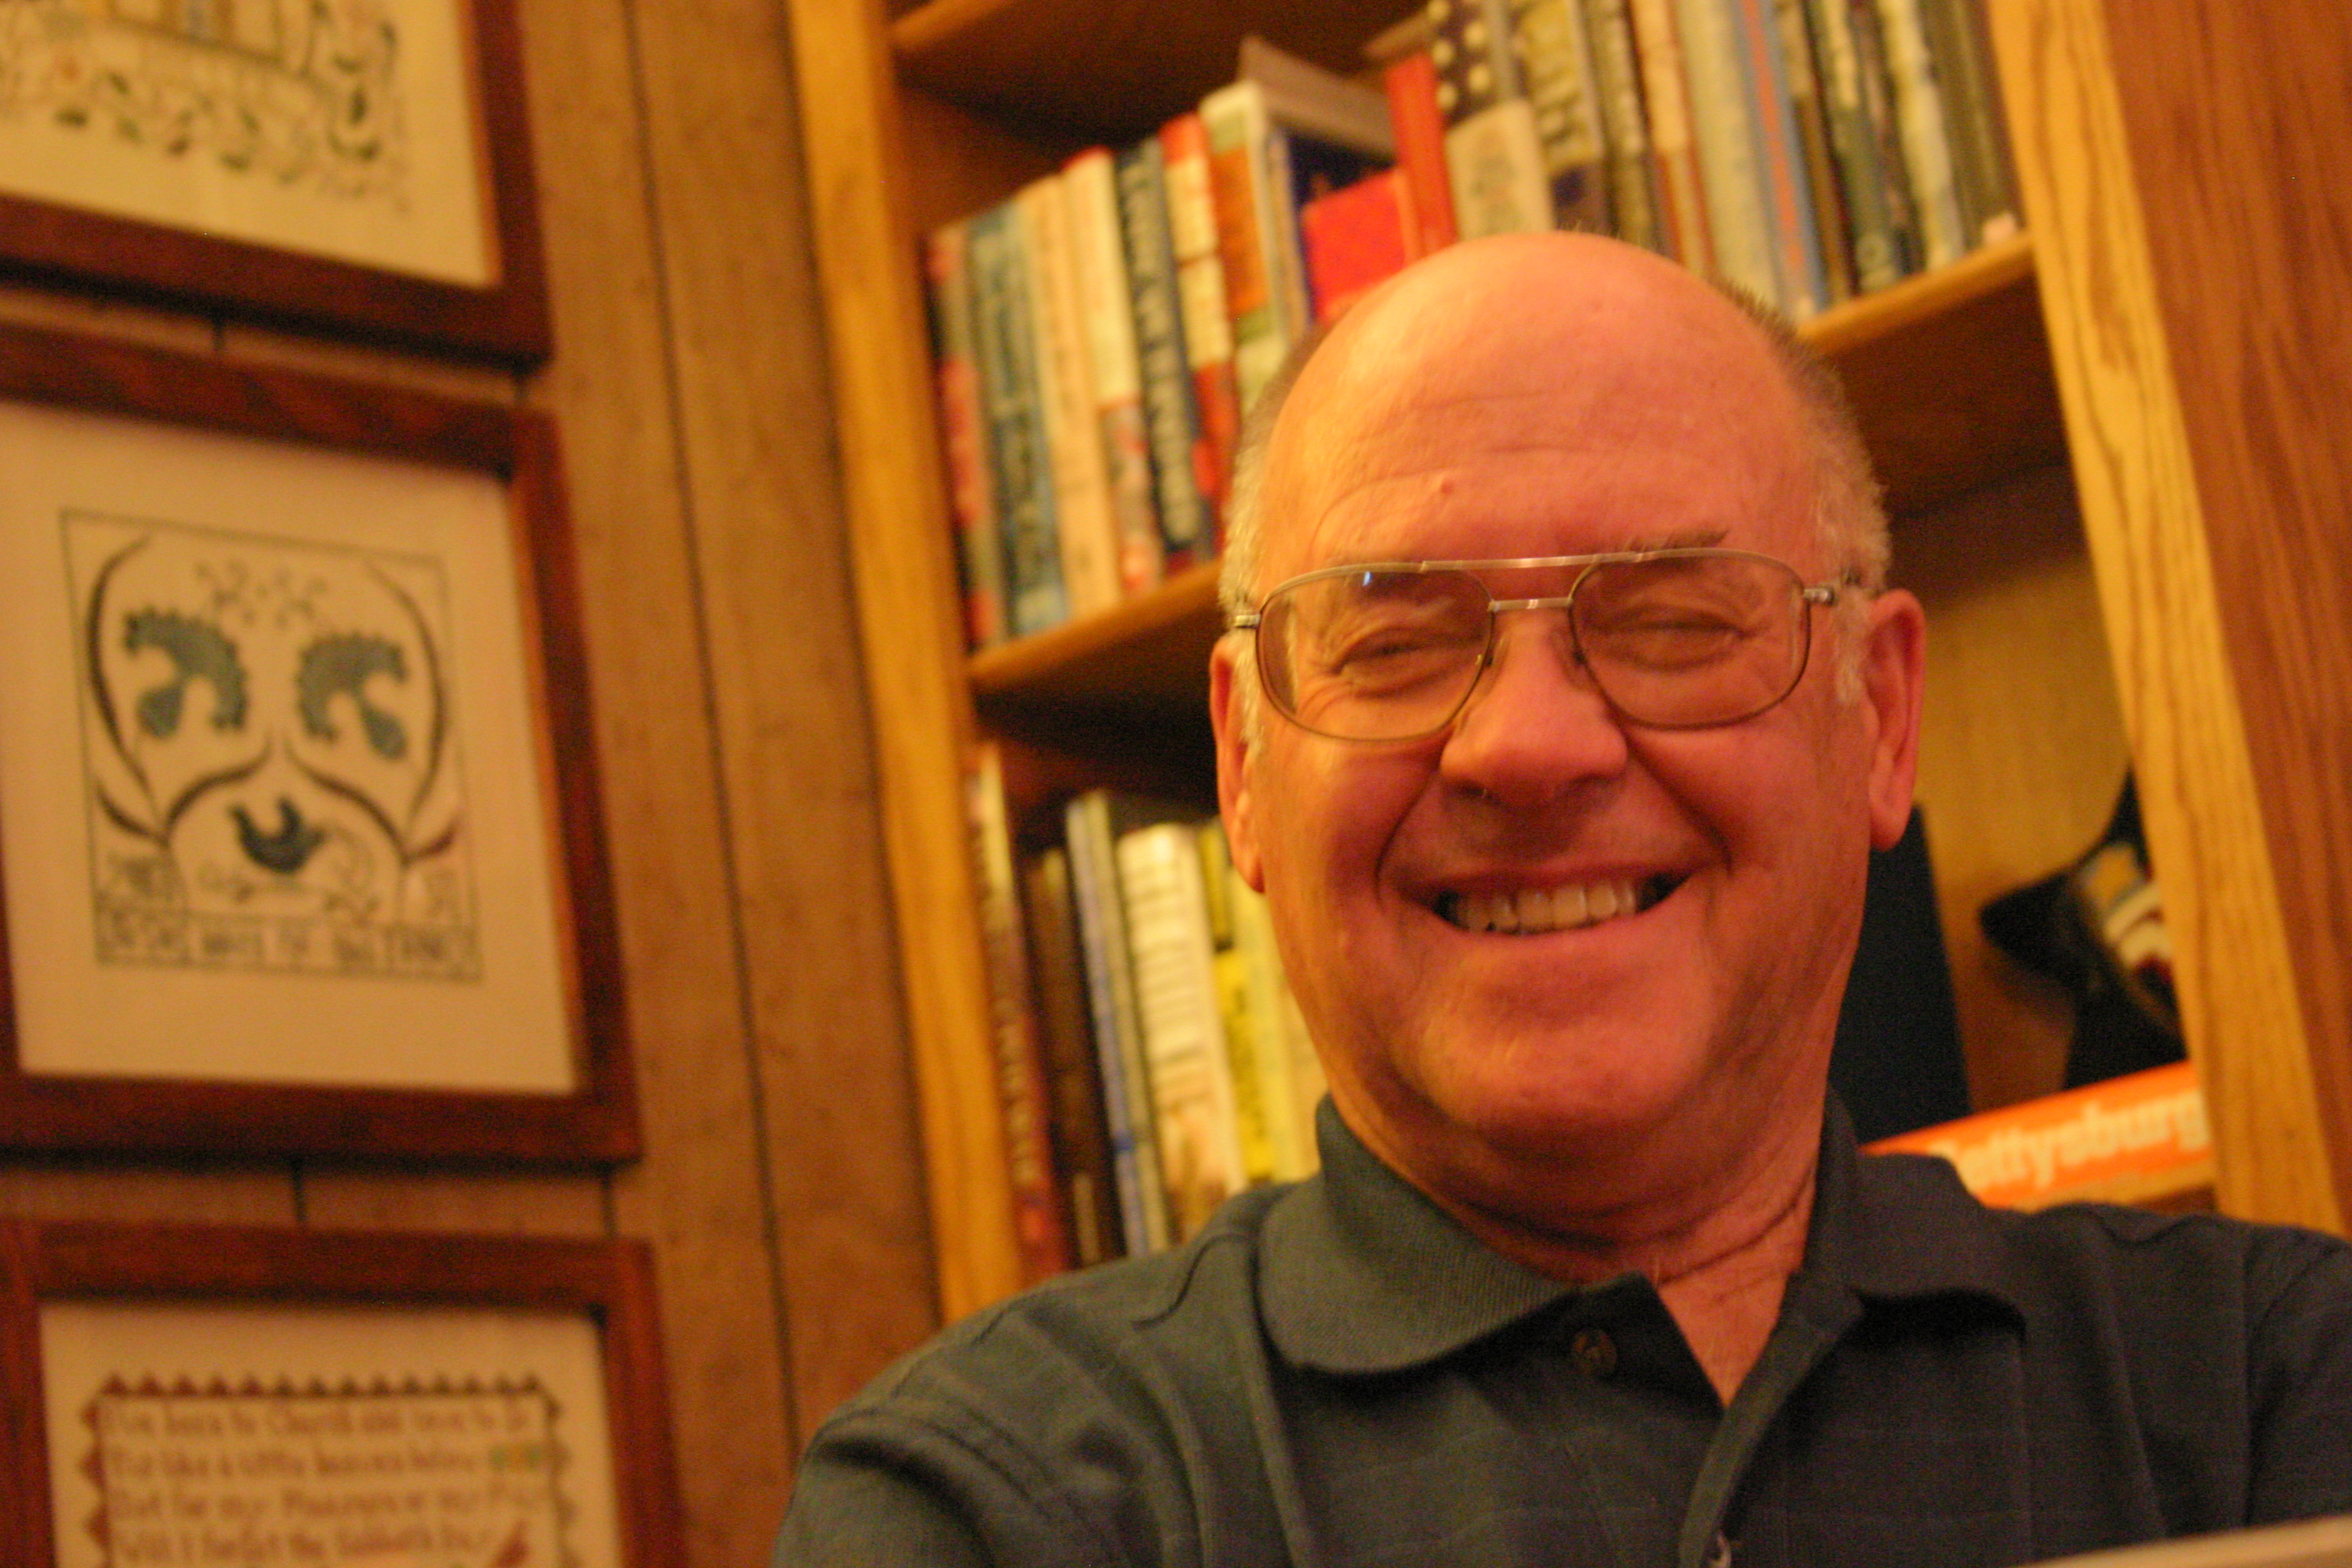
\includegraphics[scale=0.05]{maurice}
  \end{center}
  \caption{Co-builder Maurice Ashby}
\label{maurice}
\end{figure}\\
\\

\newpage
\section{Appendix}
All code and schematics are released under the Creative Commons Attribution-Noncommercial 3.0 United States License.\\
The code can be found online at github: http://github.com/JoshAshby/Robotbob/tree/experimental\\
Source for this \LaTeX ~{}PDF can be found online at github: http://github.com/JoshAshby/BOB-Documentation\\

\lstinputlisting[caption={Adc.c},label=adc,frame=bl]{../adc.c}
\lstinputlisting[caption={Pwm.c},label=pwm,frame=bl]{../pwm.c}
\lstinputlisting[caption={Digital.c},label=digital,frame=bl]{../digital.c}
\lstinputlisting[caption={Boot.c},label=boot,frame=bl]{../boot.c}
\lstinputlisting[caption={Robot.c},label=robotfunc,frame=bl]{../robotfunc.c}
\lstinputlisting[caption={Global.h},label=global,frame=bl]{../global.h}
\lstinputlisting[caption={Version.h},label=version,frame=bl]{../version.h}

\end{document}
